\documentclass[../main.tex]{subfiles}
\begin{document}
\newpage
\hypertarget{q15}{\section{Площадь криволинейного сектора, пример для лемнискаты Бернулли.}}
\begin{example}[Площадь криволинейного сектора]
    
    ~

    Криволинейный сектор можно определить как множество точек, ограниченное углом и некоторой кривой - функцией от угла. В полярной системе координат это можно описать как 
    \[ E=\left\{ \left( \varphi , \rho\right): \; \varphi \in \left[ a , b \right],\; 0 \leq \rho \leq r\left( \varphi \right)\right\}\]
    где \( r\left( \varphi \right) \in C\left[ a , b \right]\) - расстояние от начала координат до ограничивающей кривой при угле \( \varphi \).

    \InsertBoxL{0}{
    \begin{minipage}[t]{7cm} 
        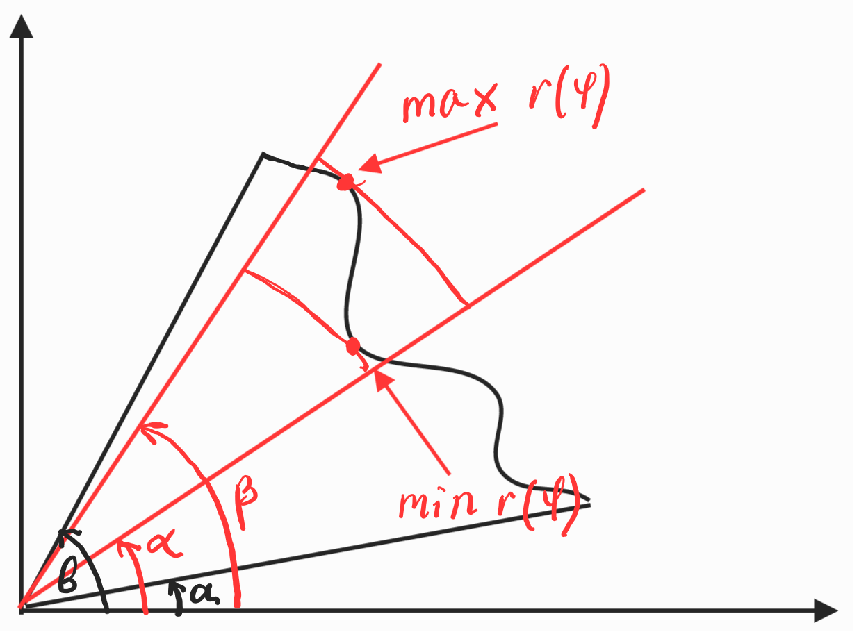
\includegraphics[width=0.98\linewidth]{15_sector.pdf} 
    \end{minipage}
    }   

    Рассмотрим аддитивную функцию промежутка \( S(\left[ \alpha , \beta \right])\) - площадь части нашего криволинейного сектора, заключённой между 
    углами \( \alpha \) и \( \beta \). Она определена на всех подотрезках отрезка \( \left[ a,b\right]\). Рассмотрим произвольный подотрезок \( \left[ \alpha , \beta \right]\).
    Площадь соответствующей части криволинейного сектора ограничивается снизу вписанным круговым сектором с радиусом, равным \( \min\limits_{ \varphi \in \left[ \alpha , \beta \right]} r\left( \varphi \right)\). 
    Она также ограничивается снизу "описанным" круговым сектором с радиусом \( \max\limits_{ \varphi \in \left[ \alpha , \beta \right]} r\left( \varphi \right)\). Поэтому мы можем написать:
    \[ \pi \left( \min\limits_{ \varphi \in \left[ \alpha , \beta \right]} r\left( \varphi \right) \right)^2\cdot \dfrac{ \beta-\alpha}{ 2 \pi } \leq S(\left[ \alpha , \beta \right]) \leq \pi \left( \max\limits_{ \varphi \in \left[ \alpha , \beta \right]} r\left( \varphi \right) \right)^2\cdot \dfrac{ \beta-\alpha}{ 2 \pi }\]

    Немного причесав эти неравенства, получим:
    \[ \min\limits_{ \varphi \in \left[ \alpha , \beta \right]} \dfrac{ (r\left(\varphi\right))^2}{ 2}\cdot \left( \beta - \alpha \right) \leq S(\left[ \alpha , \beta \right]) \leq \max\limits_{ \varphi \in \left[ \alpha , \beta \right]} \dfrac{ (r\left(\varphi\right))^2}{ 2}\cdot \left( \beta - \alpha \right)\]

    И так как это верно \( \forall \; \left[ \alpha , \beta \right] \subseteq  \left[ a,b\right]\), \hyperlink{density_thm}{по признаку плотности} \( \dfrac{ (r\left(\varphi\right))^2}{ 2}\) - плотность функции \( S\). Поэтому
    \[ \boxed{ S\left( \left[ a,b\right]\right)= \dfrac{ 1}{ 2}\displaystyle\int\limits_{ a}^{ b}\left( r\left( \varphi \right)\right)^2d \varphi }\]
\end{example}

\begin{example}[Площадь лемнискаты Бернулли]
    
    ~

    \InsertBoxL{0}{
    \begin{minipage}[t]{6cm} 
        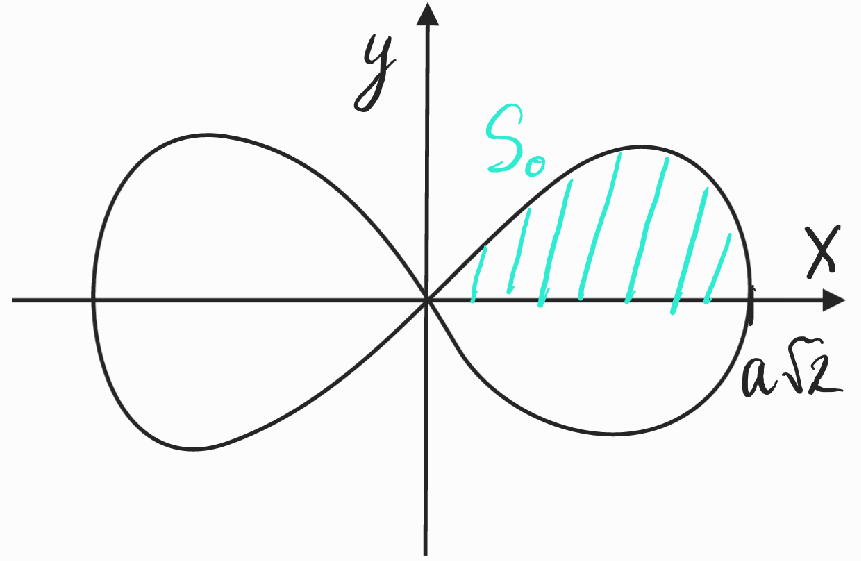
\includegraphics[width=0.98\linewidth]{15_lemniscata.pdf} 
    \end{minipage}
    }   

    Лемниската Бернулли - это кривая, которая в полярных координатах задаётся уравнением \( r = a \;\sqrt[]{2 \cos \left( 2 \varphi \right)}\). 
    Мы хотим найти площадь, которую эта кривая ограничивает. Сначала немного преобразуем равенство:
    \[ r^2 = 2a^2 \cos\left( 2 \varphi \right)\]
    \begin{equation}\label{eq:lemniscata}
        r^4=r^2 \cdot r^2=2a^2\cos\left( 2 \varphi \right)\cdot r^2=2a^2\left( r^2\cos ^2 \varphi - r^2\sin^2 \varphi \right)
    \end{equation}

    Полярная и декартова системы координат связаны друг с другом так: 
    \begin{equation*}
        \begin{cases}
            x=r\cos \varphi \\ 
            y=r\sin \varphi 
        \end{cases}
        \implies 
        \begin{cases}
            r^2\cos^2 \varphi =x^2\\
            r^2\sin^2 \varphi =y^2\\ 
            x^2+y^2=r^2\left( \cos^2 \varphi +\sin^2 \varphi \right)=r^2 \implies r^4=\left( x^2+y^2\right)^2
        \end{cases}
    \end{equation*}

    Подставим это в равенство \ref{eq:lemniscata}, получим: 
    \[ (x^2+y^2)^2=2a^2\left( x^2-y^2\right)\]

    Из этого уравнения видно, что кривая симметрична относительно осей \( x\) и \( y\) (если поставить \( -x\) вместо \( x\) или \( -y\) вместо \( y\) будет то же самое). Поэтому мы будем искать площадь \( S_0\) только той части кривой, которая 
    лежит в первой координатной четверти, то есть там где \( \varphi \in \left[ 0, \dfrac{ \pi}{ 2}\right]\), а потом умножим её на 4 и получим полную площадь \( S\).
    \begin{equation*}
        \begin{cases}
            \varphi \in \left[ 0, \dfrac{ \pi}{ 2}\right]\\
            \cos 2 \varphi \geq 0
        \end{cases}
        \implies 
        \varphi \in \left[ 0, \dfrac{ \pi}{ 4}\right]
    \end{equation*}

    У нас есть промежуток, в пределах которого меняется угол \( \varphi \), есть функция \( r\left( \varphi \right)\), которая задаёт кривую. Значит
    для расчёта площади мы можем использовать формулу площади криволинейного сектора. 

    \[ S_0= \dfrac{ 1}{ 2} \displaystyle\int\limits_{ 0}^{ \frac{ \pi}{ 4}} 2a^2\cos\left( 2 \varphi \right)d \varphi =a^2 \displaystyle\int\limits_{ 0}^{ \frac{ \pi}{ 4}} \cos \left( 2 \varphi \right)d \varphi = a^2\left( \dfrac{ 1}{ 2} \sin\left( 2 \varphi \right)|_{0}^{\frac{ \pi}{ 4}}\right) = \dfrac{ a^2}{ 2}\]

    \[ \boxed{S=2a^2}\]
\end{example}
\end{document}